\documentclass{hw}
\usepackage[version=4]{mhchem}
\usepackage{nuc}
\usepackage[load=addn]{siunitx}
\usepackage{amsmath}
\usepackage{cancel}
\usepackage{physics}
\usepackage{booktabs}
\usepackage{hyperref}
\graphicspath{ {images/}}

\DeclareSIUnit\eVperc{\eV\per\clight}
\DeclareSIUnit\year{yr}

\author{J.R. Powers-Luhn}
\date{2016/11/17}
\title{Homework Chapter 10}

\begin{document}

\problem{}
$\ce{^{147}Pm}$ is a pure beta emitter with a \SI{2.6234}{\year} half life. By 
using radioactive seeds, a radioisotope can be evenly distributed in a tumor 
site. Assume a tumor site with a density of \SI{1}{\gram\per\centi\meter^3} 
and a mass of \SI{11}{\gram}. If the plan is to deliver \SI{25}{\gray} of dose 
to the entire prostate, calculate the activity of the $\ce{^{147}Pm}$ at the 
time of implantation into the prostate. Assume it has a biological half life 
similar to $\ce{^{131}I}$.

\solution
Decay information was obtained from 
\url{http://nucleardata.nuclear.lu.se/toi/nuclide.asp?iZA=610147}
See calculations in attached code. Assuming all of the activity is captured in 
the prostate, the activity required is:

\begin{align*}
A &= D m \frac{\lambda_b + \lambda_p}{E} \\
&= \SI{5.10e5}{\gray}
\end{align*}

\problem{}
\SI{1e-6}{\gram} of $\ce{^{59}Co}$ is placed into the high flux reactor at 
ORNL. After 24 days of irradiation, what is the activity of $\ce{^{60}Co}$ in 
the sample? How many atoms of $\ce{^{59}Co}$ have been lost in that time 
period? Use a flux of \num{1e15} thermal neutrons 
\si{\per\centi\meter^2\per\second}.

\solution
Cross section obtained from the BNL Sigma page at \url{http://www.nndc.bnl.gov/sigma/index.jsp?as=59&lib=endfb7.1&nsub=10}. Calculations were performed in the attached code. From Turner, equation 4.40, the concentration of $\ce{^{60}Co}$ is:

\begin{align*}
N_{60} &= \frac{\lambda_{59} N_{59}}{\lambda_{60} - \lambda_{59}} \left( \e^{-\lambda_{59} t} - \e^{-\lambda_{60} t} \right) \\
\intertext{Substituting the removal term $\phi \sigma_{59}$ for $\lambda_{59}$}
&= \frac{\phi \sigma_{59} N_{59}}{\lambda_{60} - \phi \sigma_{59}} \left( \e^{-\phi \sigma_{59} t} - \e^{-\lambda_{60} t} \right) \\
&= \SI{2.87e6}{\becquerel}
\end{align*}

\problem{}
What fluence of neutrons from a DT generator ($\ce{d + t \rightarrow n + 
^{4}He}$) is required to deliver a KERMA of \SI{1}{\gray}?

\solution
Anderson Appendix 10 lists values for Kerma per fluence of neutrons in water. The energy of neutrons from a DT generator is \SI{14.1}{\mega\electronvolt}. Interpolating between \SI{10}{\mega\electronvolt} and \SI{15}{\mega\electronvolt} (see attached code) and solving, we get:

\begin{align*}
\phi &= \frac{K}{K / \phi} \\
&= \SI{1.45e6}{\per\meter^2}
\end{align*}

\problem{Anderson 10.11}
The linear attenuation coefficient for $\ce{^{60}Co}$ radiation in water is 
\SI{6.5}{\per\meter}.
\begin{enumerate}
    \item Calculate the dose at points at depths \SI{0.01}{\meter}, 
    \SI{0.05}{\meter}, \SI{0.1}{\meter}, \SI{0.2}{\meter} along the central 
    axis for $F$ of \SI{0.8}{\meter}. Assume the maximum dose is 
    \SI{100}{\rad}. Ignore scatter.
    \item Compare your calculations with the measured values in Appendix 11 
    for a $10 \times 10$ \si{\centi\meter} field. Calculate the dose 
    attributable to scatter and the buildup factor at each depth.
\end{enumerate}

\solution
\part
Calculations performed in attached code. From Anderson equation 10.22:

\begin{align*}
D(d, F, A/P) = D(d_m, F, A/P) \frac{BF(d, A/P)}{BF(d_m, A/P)} \left[ \frac{F + d_m}{F + d} \right]^2 \exp{-\mu_{eff} (d - d_m)} \numberthis \label{eqn:10.22}
\end{align*}

From Appendix 11, we determine that, since at $d = \SI{0.5}{\centi\meter}$, $BF=1$, $d_m = \SI{0.5}{\centi\meter}$. We ignore the $BF$ terms and calculate:

\begin{tabular}{ccccc}
\toprule
Depth (\si{\meter}) &  Calculated &  Measured &        BF &  BS Dose Contribution \\
\midrule
0.01 &   95.610844 &      98.2 &  1.027080 &              2.589156 \\
0.05 &   66.945713 &      78.5 &  1.172592 &             11.554287 \\
0.10 &   43.144943 &      55.6 &  1.288679 &             12.455057 \\
0.20 &   18.244145 &      27.2 &  1.490889 &              8.955855 \\
\bottomrule
\end{tabular}


\part
Comparison with the values in Appendix 11 was performed in the table above and graphically in figure \ref{fig:dose}. The difference between the two was attributed to the backscatter terms that were neglected in equation \ref{eqn:10.22}.

\begin{figure}[h]
	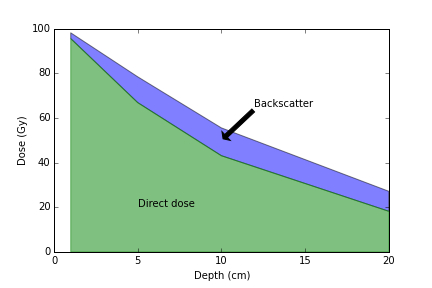
\includegraphics[width=15cm,height=10cm,keepaspectratio]{problem4}
	\caption{Dose contribution from direct and BS}
	\label{fig:dose}
\end{figure}

\end{document}